\section{Background and Related Work}\label{sec:related}

\subsection{Datasets}\label{sec:data}
Three public datasets are used. \emph{MOT17} \cite{milan2016mot16} contains 14 sequences of
people filmed with static and moving cameras. As is common, the second half of each of the seven
training sequences, called val-half (2,652 frames), is used for evaluation \cite{zhang2022bytetrack},
with the published YOLOX-X detections \cite{ge2021yolox} at the two published emission floors, the
lowest scores emitted, of 0.01 and 0.1. To study score changes directly, these scores were also
changed before the tracker by four transforms that keep their order: cubing ($s^3$), halving
($0.5\,s$), and logit temperatures $T=2$ and $T=0.5$, which divide the logit (log-odds, Sect.~\ref{sec:problem}) of each score by $T$.
\emph{KITTI tracking} \cite{geiger2012kitti} has 21 training sequences (8,008 frames) recorded from
a car and is scored on cars and pedestrians; here the trackers run with two other detectors,
YOLOv8n \cite{jocher2023yolov8} and RT-DETR-L \cite{zhao2024rtdetr}, and keep thresholds that were
set for other detectors. \emph{UAVDT} \cite{du2018uavdt} contains drone videos of vehicles; its 20
test sequences (16,592 frames) are used with ByteTrack, YOLOv8n, and RT-DETR-L.

MOT17 with four trackers, KITTI, and the score transforms were development data, looked at while
\scl{} was designed. Two predeclared external trackers, PD-SORT and Hybrid-SORT, were chosen in
advance and run once with the frozen configuration on the detections released by their authors on
MOT17 val-half. The held-out UAVDT test split was also run once, after a written plan. Each
external host was checked against its authors' number: EXACT within 0.2 HOTA points, CLOSE within
1.0.

\subsection{Evaluation metrics}\label{sec:metrics}
HOTA \cite{luiten2021hota}, the main metric, balances finding the objects and keeping their
identities,
\begin{equation}
\mathrm{HOTA}=\frac{1}{19}\sum_{\alpha}\sqrt{\mathrm{DetA}_\alpha\,\mathrm{AssA}_\alpha},
\label{eq:hota}
\end{equation}
where $\mathrm{DetA}_\alpha$ and $\mathrm{AssA}_\alpha$ are the detection and association accuracy
at the localization threshold $\alpha=0.05,0.10,\dots,0.95$. MOTA \cite{bernardin2008clear} and
IDF1 \cite{ristani2016idf1} are
\begin{align}
\mathrm{MOTA}&=1-\frac{\mathrm{FN}+\mathrm{FP}+\mathrm{IDS}}{\mathrm{GT}},\label{eq:mota}\\
\mathrm{IDF1}&=\frac{2\,\mathrm{IDTP}}{2\,\mathrm{IDTP}+\mathrm{IDFP}+\mathrm{IDFN}},\label{eq:idf1}
\end{align}
where FN are missed objects (false negatives), FP false positives, IDS identity switches (an
object's ID changes), and GT the number of ground-truth boxes; IDTP, IDFP, and IDFN count boxes
after each ground-truth track is matched to at most one output track. All metrics are computed
with TrackEval (commit 12c8791) and the official ground truth \cite{dendorfer2021motchallenge};
KITTI HOTA is averaged over cars and pedestrians, and on UAVDT all vehicles form one class and
predictions in ignored regions are removed. HOTA, MOTA, and IDF1 are in percent, and differences
in points.

All comparisons are paired: each tracker runs alone and with \scl{} on the same sequences and
detections. Paired bootstrap resampling of whole sequences \cite{efron1993bootstrap}, 10,000 times
with seed 42, gives a 95\% interval (2.5--97.5 percentiles) for each difference, which is called
significant when its interval does not include zero.

\subsection{Related work}\label{sec:survey}
\emph{Tracking by detection.}\label{sec:hosts} SORT matches Kalman-filter predictions to new
detections by their overlap \cite{bewley2016sort}; ByteTrack added a second step that uses
low-score detections to continue tracks \cite{zhang2022bytetrack}; OC-SORT uses one score
threshold \cite{cao2023ocsort}. Their thresholds were tuned for one detector, usually YOLOX
\cite{ge2021yolox}. Many recent trackers improve association with trained or domain-specific
parts \cite{li2024fdbtrack,bao2024graphmatching,zhang2025sinkhorn,ding2025remot,liang2024motiontrack,sun2026bsr},
which change or retrain the tracker; \scl{} keeps both the tracker and the detector unchanged.
Seven published trackers serve as hosts in this study, each with the authors' code and published
configuration: ByteTrack, BoT-SORT \cite{aharon2022botsort}, OC-SORT, SparseTrack
\cite{liu2025sparsetrack}, BoostTrack \cite{stanojevic2024boosttrack}, PD-SORT
\cite{wang2025pdsort}, and Hybrid-SORT \cite{yang2024hybridsort}. ByteTrack is used with the
thresholds that its authors used on MOT17 (official setting) and with the defaults of the
Ultralytics library, which also provides BoT-SORT (library setting).

\emph{Adaptive thresholds.} Adaptive ByteTrack sets ByteTrack's threshold from each frame
\cite{ma2023adaptivebytetrack}, AdapTrack adapts its matching thresholds \cite{shim2024adaptrack},
and ACT sets the high and low thresholds from the first quartile and the number of the current
scores \cite{act2026adaptive}. ConfTrack weights the Kalman update and the matching cost by the
score \cite{jung2024conftrack}, and PlugTrack blends motion predictors with a trained network
\cite{kim2026plugtrack}.

\emph{Comparison.} Table~\ref{tab:compare} compares \scl{} with the adaptive-thresholding and
score-calibration methods. The adaptive-thresholding methods act in every frame, read only the
current frame or each box, and are built into one tracker; calibration acts on every score and
needs labelled data. \scl{} differs in three ways. It is selective: it first decides, from the
scores of past frames, whether to act at all, and leaves a well-matched tracker as it is. It is
host-aware: it reads the tracker's published settings and serves several unchanged single-stage
and two-stage trackers through them. And it needs neither labels nor trained parts; its new scores
encode decisions for the tracker's thresholds rather than calibrated probabilities
(Sect.~\ref{sec:choice}). It is also tested as one frozen configuration under score changes and on
external systems, and against ACT on the same detections (Sect.~\ref{sec:baselines}).

\begin{table*}[!tp]
\caption{\scl{} compared with adaptive-thresholding and score-calibration methods. Each row is one method; the columns give what it changes, what information it uses, whether it needs labels or trained parts, when it acts, and where it runs. ReID: re-identification network.}
\label{tab:compare}
\centering\footnotesize
\setlength{\tabcolsep}{3pt}
\begin{tabular}{@{}>{\raggedright\arraybackslash}p{23mm}>{\raggedright\arraybackslash}p{28mm}>{\raggedright\arraybackslash}p{28mm}>{\raggedright\arraybackslash}p{19mm}>{\raggedright\arraybackslash}p{24mm}>{\raggedright\arraybackslash}p{25mm}@{}}
\toprule
Method & What is adapted & Information used & Labels or trained parts & When it acts & Where it works\\
\midrule
\multicolumn{6}{@{}l}{\textit{Adaptive thresholding}}\\
Adaptive ByteTrack \cite{ma2023adaptivebytetrack} & high/low score split & scores of the current frame & none & every frame & inside ByteTrack\\
AdapTrack \cite{shim2024adaptrack} & matching thresholds & current frame & ReID network & every frame & its own tracker\\
ACT \cite{act2026adaptive} & high and low thresholds, chosen from preset levels & first quartile and number of the current scores & none & every frame & inside the tracker\\
ConfTrack \cite{jung2024conftrack} & Kalman update and matching cost & score of each box & ReID network & every box & its own tracker\\
\addlinespace[3pt]
\multicolumn{6}{@{}l}{\textit{Score calibration}}\\
K{\"u}ppers et al.\ \cite{kuppers2020detcalib} & detector scores, mapped to probabilities & labelled data & calibration map & every score & detector output\\
\addlinespace[3pt]
\multicolumn{6}{@{}l}{\textit{This paper}}\\
\scl{} & candidates, scores, thresholds, matching tolerance & logits of past frames; host contract & none & only when the scores are noisy (clean: thresholds capped) & between a detector and unchanged trackers\\
\bottomrule
\end{tabular}
\end{table*}


\begin{figure*}[t]
\centering
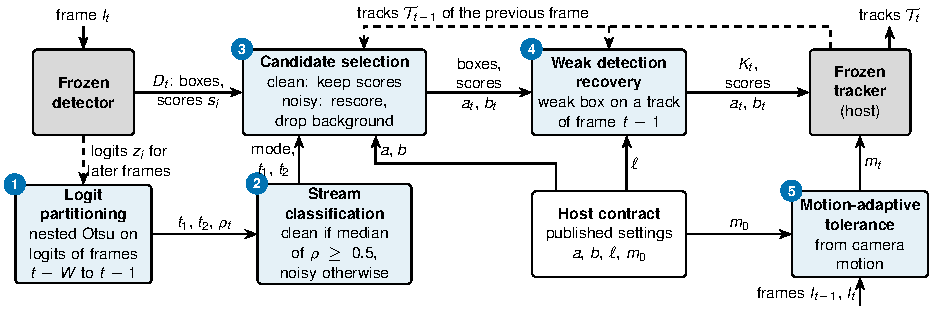
\includegraphics{Fig1.pdf}
\caption{\scl{} between a frozen detector and a frozen tracker (the host), for frame $t$. Each
arrow is labelled with the data it carries; dashed arrows carry data kept from earlier frames.
Steps 1--5 are described in Sects.~\ref{sec:calib}--\ref{sec:motion}, and the host contract in
Sect.~\ref{sec:contract}; every symbol is explained in Table~\ref{tab:symbols}}
\label{fig:arch}
\end{figure*}

\emph{Score calibration and adaptive inference.} Detector families such as YOLOX, YOLOv8, and RT-DETR give different score distributions,
and calibration methods learn a mapping from labelled data \cite{kuppers2020detcalib}. Otsu's
method picks, without labels, the threshold that best splits a histogram into two groups
\cite{otsu1979}; \scl{} applies it to the logits of recent scores. Dynamic networks learn their
settings for each model \cite{han2022dynamic}, and a separate controller, AC-MOT (submitted), sets the detector operating point from
image and track cues. \scl{} instead reads the scores and acts on the tracker's input and
thresholds.
